
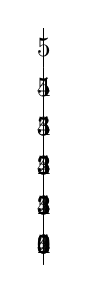
\begin{tikzpicture}
	\foreach \n  in {0, ..., 5} {
			\foreach \f in {0,...,\n}{
					\tikzmath{
						\finger = 0.7;
						\x = \n - \f * \finger;
					};

					\draw (\x, \f / 2) rectangle node {$\n$} (\x + 1, \f / 2 + 0.5);
				};
		};
\end{tikzpicture}